\documentclass[12pt,a4paper]{article}

\usepackage[T1]{fontenc}
\usepackage[utf8]{inputenc}
\usepackage[brazil]{babel}
\usepackage{graphicx}
\usepackage{geometry}
\usepackage{listings}
\usepackage{listingsutf8}
\usepackage{xcolor}
\usepackage{setspace}
\usepackage{float}
\usepackage{tikz}
\usepackage{tabularx}

\usetikzlibrary{positioning, shapes.geometric}
\onehalfspacing
\geometry{margin=2.5cm}

\lstset{
    language=SQL,
    basicstyle=\ttfamily\small,
    keywordstyle=\color{blue},
    commentstyle=\color{gray},
    stringstyle=\color{red},
    breaklines=true,
    showstringspaces=false
}

\newcommand{\montarinicio}[3]{
    % =========================
    % CAPA
    % =========================
    \begin{titlepage}
        \centering

        {\large Faculdade Anhanguera}\\[0.5cm]
        {\large Tecnólogo em DevOps}\\[3cm]

        {\Large \textbf{#1}}\\[2cm]

        {\large Gabriel Blank Stift Mousquer}\\[1cm]

        {\large Ivoti/RS}\\
        {\large 2026}

    \end{titlepage}

    % =========================
    % FOLHA DE ROSTO
    % =========================
    \begin{titlepage}
        \centering

        {\large Faculdade Anhanguera}\\[0.5cm]
        {\large Tecnólogo em DevOps}\\[2cm]

        {\Large \textbf{#1}}\\[1.5cm]

        \begin{flushright}
            Trabalho apresentado à disciplina de \\
            \textbf{#2} \\
            Professor: #3 \\
        \end{flushright}

        \vfill

        {\large Gabriel Blank Stift Mousquer}\\
        Matrícula: 2024201126\\

        \vfill

        {\large Ivoti/RS}\\
        {\large 2026}

    \end{titlepage}

    % =========================
    % SEÇÃO: TOC
    % =========================
    \tableofcontents
    \newpage
}


\begin{document}

\montarinicio
    {TRABALHANDO COM UMA TABELA NO BANCO DE DADOS}
    {Programação e Desenvolvimento de Banco de Dados}
    {Thaysla Fernanda Da Cruz Cardoso}

% =========================
% SEÇÃO: INTRODUÇÃO
% =========================
\section{Introdução}

O presente trabalho tem como objetivo demonstrar a utilização de comandos da linguagem SQL no contexto de manipulação e modificação de dados em bancos de dados relacionais, conforme proposto na atividade prática. Em particular, busca-se compreender e aplicar instruções de inserção, atualização e exclusão de registros, bem como comandos de definição de dados (DDL) para alteração da estrutura de tabelas.

Além disso, são abordadas modificações estruturais na tabela \texttt{funcionarios}, incluindo a adição e remoção de colunas e a alteração de tipos de dados. Também é explorada a aplicação de constraints, com ênfase na utilização da restrição \texttt{UNIQUE} para garantir a integridade dos dados armazenados.

As atividades foram realizadas em um ambiente baseado no sistema operacional \textit{Ubuntu 24.04.4 LTS}, utilizando o sistema gerenciador de banco de dados \textit{MySQL}, versão 8.0.45, acessado por meio de sua interface de linha de comando (CLI).

Para a execução dos comandos, foi utilizado um usuário específico, denominado \texttt{aula1}, criado exclusivamente para a realização das operações propostas. O acesso ao banco de dados foi efetuado via terminal, utilizando o comando \texttt{mysql -u aula1 -p}.

A partir desse ambiente, foram executadas as etapas previstas no exercício, incluindo a manipulação de dados, alterações estruturais na tabela e aplicação de restrições, conforme detalhado nas seções seguintes.

% =========================
% SEÇÃO: DESENVOLVIMENTO
% =========================
\section{Desenvolvimento}

Inicialmente, foram inseridos novos registros na tabela \texttt{funcionarios}, incluindo informações de nome, departamento e salário, conforme apresentado na Figura~\ref{fig:inserir-funcionarios}.

\begin{figure}[H]
    \centering
    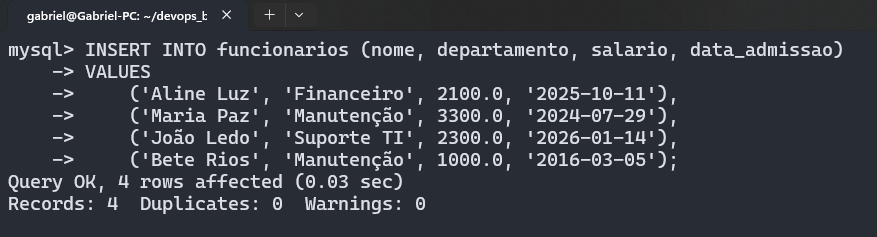
\includegraphics[width=0.8\textwidth]{./static/1-inserir-funcionarios.png}
    \caption{Inserção de funcionários}
    \label{fig:inserir-funcionarios}
\end{figure}

Em seguida, foi realizada a atualização do salário de um funcionário específico, aplicando um reajuste percentual sobre o valor previamente armazenado, como mostrado na Figura~\ref{fig:atualizar-salario}.

\begin{figure}[H]
    \centering
    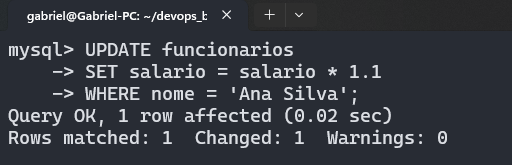
\includegraphics[width=0.8\textwidth]{./static/2-atualizar-salario.png}
    \caption{Atualização do salário do funcionário}
    \label{fig:atualizar-salario}
\end{figure}

Posteriormente, foram removidos registros de funcionários com base no departamento ao qual pertenciam, conforme ilustrado na Figura~\ref{fig:excluir-funcionarios}.

\begin{figure}[H]
    \centering
    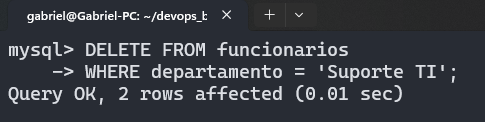
\includegraphics[width=0.8\textwidth]{./static/3-excluir-funcionarios.png}
    \caption{Exclusão de funcionários}
    \label{fig:excluir-funcionarios}
\end{figure}

Também foram realizadas alterações na estrutura da tabela, incluindo a adição de uma nova coluna para armazenamento de e-mail, a modificação do tipo de dados da coluna de salário e a remoção de um atributo previamente existente, conforme apresentado na Figura~\ref{fig:alterar-colunas}.

\begin{figure}[H]
    \centering
    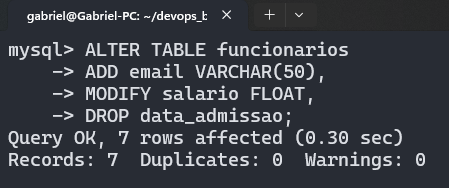
\includegraphics[width=0.8\textwidth]{./static/4-alterar-colunas.png}
    \caption{Modificação das colunas da tabela}
    \label{fig:alterar-colunas}
\end{figure}

Por fim, foi aplicada uma constraint do tipo UNIQUE à coluna \texttt{email}, restringindo a inserção de valores duplicados nesse campo, como pode ser observado na Figura~\ref{fig:adicionar-constraint}.

\begin{figure}[H]
    \centering
    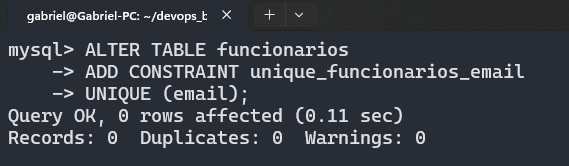
\includegraphics[width=0.8\textwidth]{./static/5-adicionar-constraint.png}
    \caption{Adição de constraint UNIQUE na coluna email}
    \label{fig:adicionar-constraint}
\end{figure}

% =========================
% SEÇÃO: CONCLUSÃO
% =========================
\section{Conclusão}

A realização da atividade permitiu aplicar, na prática, operações de inserção, atualização e exclusão de dados, bem como alterações na estrutura de tabelas e definição de constraints em um banco de dados relacional.

Durante o desenvolvimento, observou-se que comandos de manipulação de dados são diretamente responsáveis pela consistência das informações armazenadas, exigindo cuidado na definição de critérios para atualização e remoção de registros. Da mesma forma, alterações estruturais, como adição e modificação de colunas, demonstram a necessidade de adaptar o banco de dados a novos requisitos sem comprometer os dados existentes.

A aplicação de constraints, como a restrição \texttt{UNIQUE}, evidenciou seu papel na prevenção de inconsistências, ao impedir a inserção de valores duplicados em campos que devem ser exclusivos, como o e-mail de funcionários.

Compreender e aplicar corretamente esses comandos é essencial, pois operações mal definidas podem resultar em perda de dados, inconsistências ou comprometimento da integridade do banco. Em sistemas reais, essas operações são realizadas continuamente, tornando necessário o domínio não apenas da sintaxe, mas também dos impactos de cada modificação realizada.

Dessa forma, a atividade contribuiu para o entendimento prático da manipulação e estruturação de dados, destacando a importância do uso adequado de comandos SQL para garantir a confiabilidade das informações em um banco de dados.

% =========================
% SEÇÃO: APÊNDICE
% =========================
\section{Apêndice}

\subsection{Script SQL completo}

\lstinputlisting[
    caption={Script SQL completo},
    label={lst:sql},
    inputencoding=utf8/latin1,
    basicstyle=\ttfamily\scriptsize
]{./static/script.sql}

\end{document}
